\documentclass[a4paper,10pt]{article}

\usepackage[utf8]{inputenc}
\usepackage{amsmath, amsfonts}
\usepackage{graphicx}
\usepackage{natbib}
\bibliographystyle{alpha}

%opening
\title{Exact kinetics of two hard discs in a rectangular box}
\author{Rosa Rodríguez \& David P.~Sanders}
%\affiliation{Departamento de Física, Facultad de Ciencias, Universidad Nacional Autónoma de México, Ciudad Universitaria, Del.~Coyoacán, México D.F. 04510, Mexico}

\usepackage{mathptmx}

\newcommand{\defeq}{:=}
\newcommand{\mean}[1]{\left \langle #1 \right \rangle}

\newcommand{\rd}{\, \mathrm{d}}

\newcommand{\RR}{\mathbb{R}}

\newcommand{\vv}{\mathbf{v}}

% \newcommand{\indicator}[1]{\mathbf{1}_{ \left \{ #1 \right \} } }
\newcommand{\indicator}[1]{\mathbf{1}_{ \{   #1 \} } } 

\setlength{\parskip}{10pt}
\setlength{\parindent}{0pt}

\begin{document}

\maketitle
\begin{abstract}
  We obtain exact results for the kinetics of the inertial motion of two hard discs in a rectangular two-dimensional box.
  In particular, we calculate exactly the mean hopping time between exchanges of the horizontal positions of the discs, as well as mean collision rates between the two discs and between the discs and the box. 
\pmb{Do we show numerically that the distributions are exponential?}
\end{abstract}

\section{Model}

We consider two discs of radius $r$ (and diameter $d=2r$) in a box of width $w$ and height $h$ (figure
\ref{billar01}. The discs move inertially in the absence of forces, following straight-line trajectories, and undergo elastic collisions with each other and with the walls of the box.

\begin{figure}
  \centering
  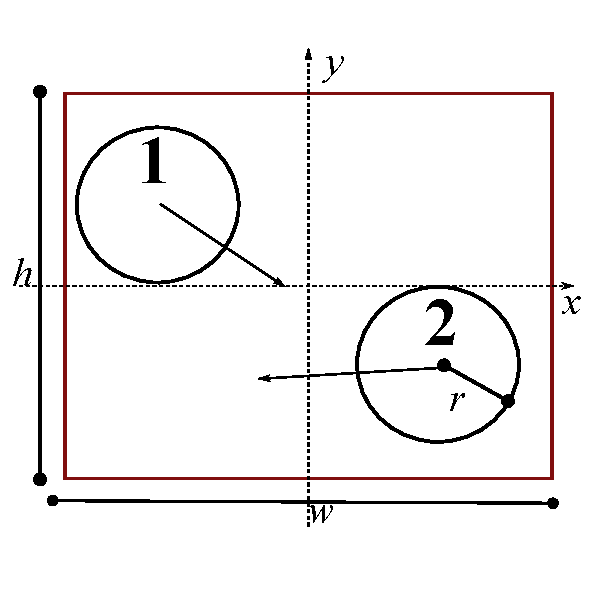
\includegraphics[width=0.56\textwidth]{DiscosenCajaCuadrada01.pdf}
  \caption{The Billiard}\label{billar01}
\end{figure}


We denote the position of the centre of the $i$th disc by $(x_{i}, y_{i})$ for $i=1,2$. Since the discs are hard, the disc centres are restricted to the region $(x_i, y_i) \in [-a,a] \times [-b, b]$, where $a \defeq a(d) \defeq \frac{w}{2} - r = \frac{w-d}{2}$ and $b \defeq b(d) \defeq \frac{h}{2} - r = \frac{h-d}{2}$.
%, and $x_i$ and $y_i$ are the Cartesian coordinates of the disc centres, with $i=1,2$.

The exclusion condition is $(x_1-x_2)^2 + (y_1-y_2)^2 \ge (2r)^2 = d^2$.
It is thus useful to work in terms of the new coordinates
\begin{equation}\label{cambiocoor01}
 x \defeq \frac{x_1 - x_2}{\sqrt{2}}; 
\quad X \defeq \frac{x_1 + x_2}{\sqrt{2}}; 
\quad y \defeq \frac{y_1 - y_2}{\sqrt{2}}; 
\quad Y \defeq \frac{y_1 + y_2}{\sqrt{2}}.
\end{equation}


In these coordinates, we have the conditions $x \in [-a \sqrt{2}, +a \sqrt{2}]$ with $X \in [-a \sqrt{2} + |x|, a \sqrt{2} - |x|]$ and similarly $y \in [-b \sqrt{2}, b \sqrt{2}]$ and $Y \in [-b \sqrt{2} + |y|, +b \sqrt{2} - |y|]$,  with the constraint $x^2 + y^2 \ge \frac{d^2}{2}$.

As sure we can notice, this defines exactly the same geometry of
the problem of two circular animals wandering in the same square territory. That is,
the exclusions define a hypercube with a cilindrical wall inside, placed
diagonaly between two hyperaristas. The dynamics in such a space
would be the usual billiard dynamics in a four dimensional table with
three dimensional borders.

\textbf{What assumption do we use for the disc collision rate?}

MAYBE NEED ANOTHER SUPPOSITION FOR DISC COLLISION RATE?

Well, it depends. If we want to calculate a \emph{Recurrence time}, then the answer is yes.
We should depart from the subset of all Outgoing trayectories frome the center of the
hypercylinder, that is, the tangent bundle of all outgoing vectors from 
the surface of the hypercilinder. If we want to calculate the FIRST encounter time, then
this supposition is not necesary, but there are no short exact ways to describe this first collision.


\section{Mean free time}

A system of $N$ hard spheres confined by hard walls inside a $d$ dimensional
space may be treated as a billiard system \cite{Sinai70, MarkChern}, 
in which a single point  particle undergoes free motion between reflecting obstacles 
in a $ d N $-dimensional configurarion space. 

If the resulting billiard is ergodic and hyperbolic, 
there is a result for the mean free time, i.e.\ the mean time between 
collisions of the particle with the walls \cite{MarkChern}. 
This can be thought of as a mean return time to the $(d-1)$-dimensional 
(i.e. codimension-$1$) cross-section given by the wall boundaries.
The formula for this is
\begin{equation}
 \mean{\tau} = \frac{|Q|}{|A|} \frac{|S^{d-1}|}{|B^{d-1}|},
\end{equation}
where the particle has velocity scaled to unity.

Here $|Q|$ denotes the $d$-dimensional volume of the available space in the billard and 
$|A|$ the $(d-1)$-dimensional area of the cross-section.
 $|S^{d-1}|$ is the $(d-1)$-dimensional area of the unit sphere in $\RR^d$ given by
\begin{equation}
  |S^{d-1}| = \frac{2 \pi^{d/2}}{\Gamma(d/2)},
\end{equation}
where $\Gamma(\cdot)$ is the gamma function. 
$|B^{d-1}|$ is the volume of the unit ball 
in $\RR^{d-1}$, given by $|B^{d-1}| = |S^{d-2}| / (d-1)$.

Machta and Zwanzig \cite{MachtaZwan} used a similar method to derive an escape 
time across a non-existent boundary by treating it as a recurrence time.
Since it is an escape time, they used velocities whose components point only 
perpendicularly to the ``exit wall''.

In our case, we are interested in the mean return time to a codimension-$1$ cross section, 
which is defined by the exact moment
in which the disk interchange their horizontal position. This is simply
\begin{equation} \label{condchoque}
x_1 = x_2.
\end{equation}
This surface is accessible from \emph{both} sides, 
so that there is an extra factor of two in the part of the velocities. Thus 
we rewrite the mean time taking this into accout: 
\begin{equation}
 \mean{\tau} = \frac{|Q| \, |S^{d-1}|} {2 \, |A| \, |B^{d-1}|}.	
\end{equation}


Given that each disk has different momentum, but
they can interchange it without affecting the
total energy, we must take into account the mass $m$ of each disk and the total kinetic energy $E$.
If both discs have the same mass $\sum_i \vv_i^2 = 2E / m$.
The above result, as derived by Chernov, was for the case $\sum_i \vv_i^2 = 1$, or $m=1$ and $E=\frac{1}{2}$.  
For more general values of $E$ and $m$, we are simply working on a different energy surface in phase space. 
The particle trajectories are identical but their motion is a factor
$\sqrt{2E/m}$ faster, so that all times are reduced by this factor, giving our version for
the mean time between events.
\begin{equation}
  \mean{\tau} = \frac{1}{\sqrt{2E / m}} 
\frac{|Q| \, |S^3|} {2 \, |A| \, |B^3|}.	
\end{equation}



\section{Calculation of volumes for the two-disc problem}

We proceed to calculate the Area and Volume quantities. From the change of coordinates,
we have a relative unconfortable geometry to work upon. The configurarion
space is an hypercube with an hypercilinder substracted in a diagona position.
The unconfortable part is to deal with the tips of the cylinder, which
present the  shape of a wedge with a circular base and two 
ortogonal ``heights''. It may be done in an indirect maner.


\subsection{Volume of available space}


We shall present the total fourdimensional volume as a product integral
of all avaible positions. To better grasp the idea, a convinient
diagram is shown in the next figure, \ref{diagintegra01}.

\begin{figure}[h]
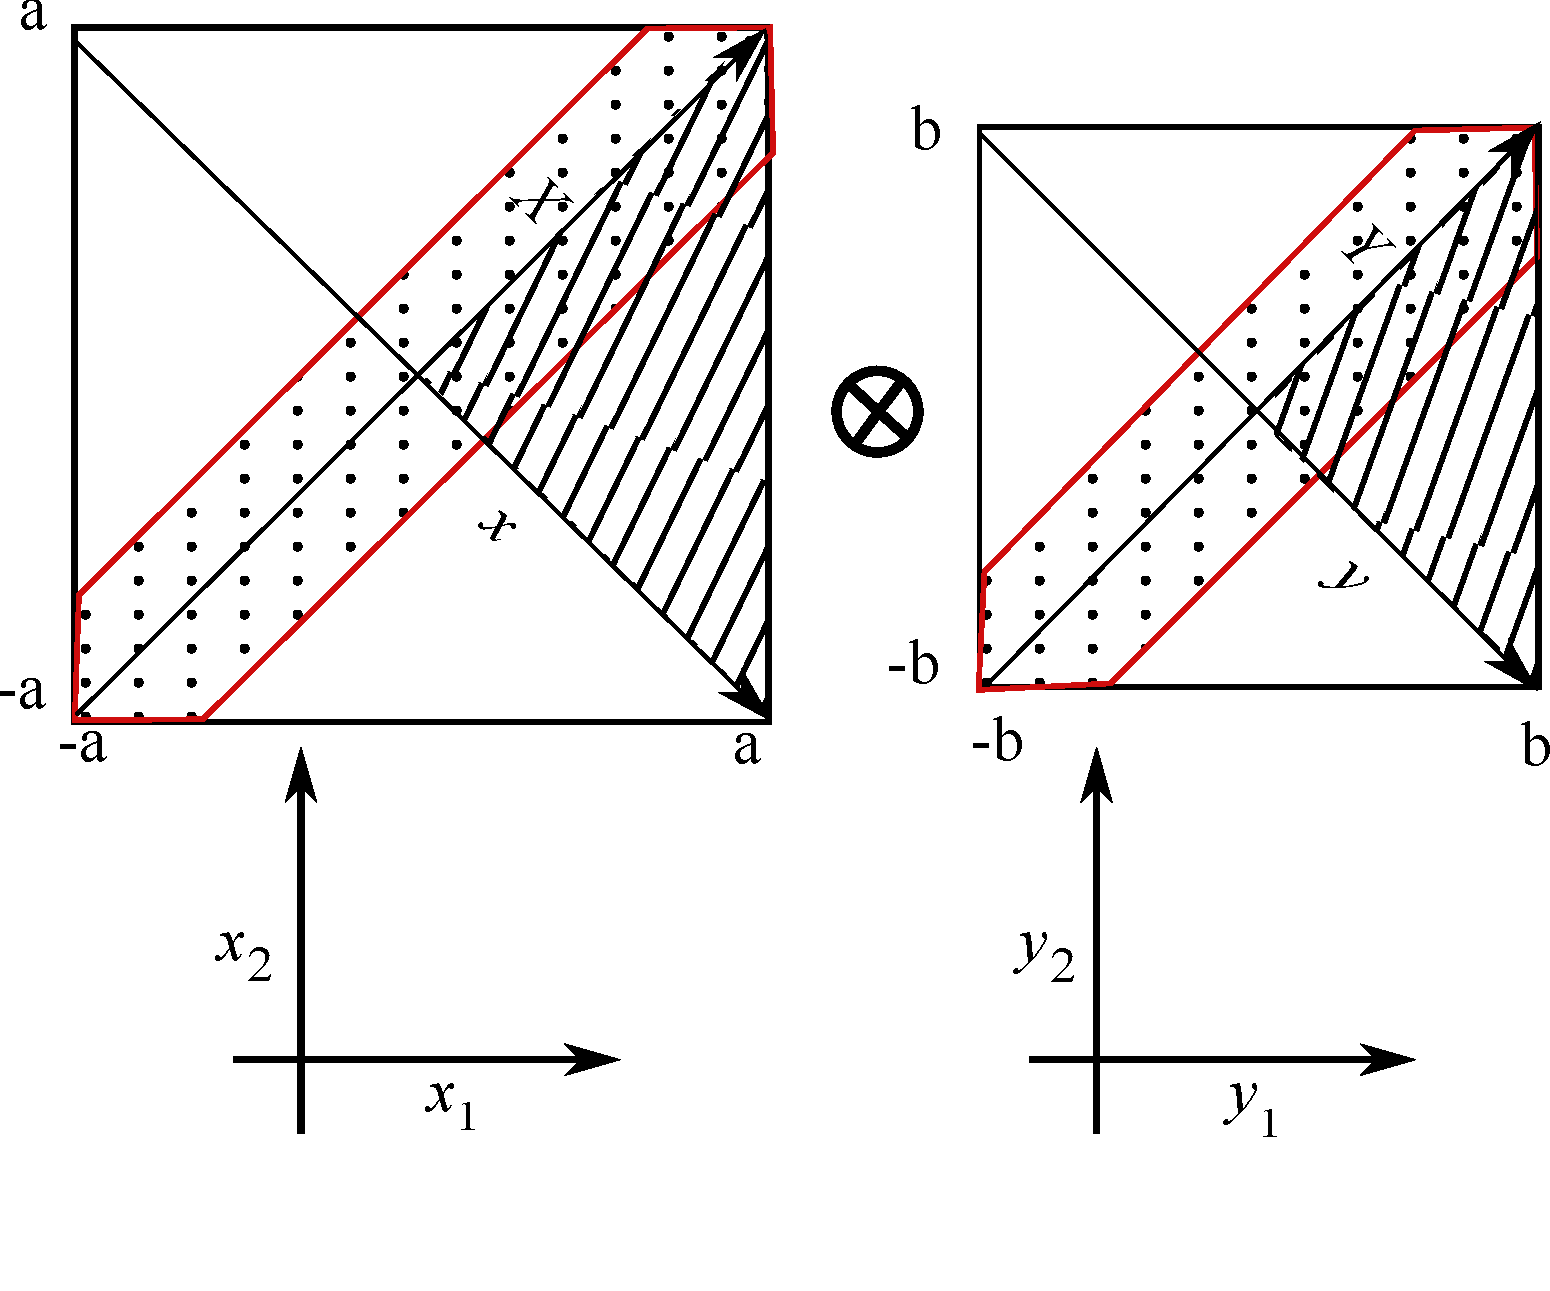
\includegraphics[width=0.8\textwidth]{diagramintegra01.pdf}
\caption{The space to integrateis the product of the subspaces
belonging to horizontal and vertical coordinates. The color
shaded area represents the ``exclusion'' set, where the condition 
$ (x_1-x_2)^2 + (y_1-y_2)^2 \ge d^2 $ is not fullfilled. 
Their width is dependent on the particular point of evaluation
on the \emph{other} subspace. The diagonal coordinates
make the expression to evaluate simpler. Due to 
symmetry, we only evaluate the area in strippes and
multiply by 16.}\label{diagintegra01}
\end{figure}

\begin{equation}
 V = \int_{x_1 = -a}^a \rd x_1 \int_{x_2 = -a}^a \rd x_2 
\int_{y_1 = -b}^b \rd y_1 \int_{y_2 = -b}^b \rd y_2 \, \indicator{ (x_1-x_2)^2 + (y_1-y_2)^2 \ge d^2 },
\end{equation}
where $\indicator{Z}$ indicates the indicator function of the set $Z$, given by $\mathbf{1}_Z (x) = 1$ if $x \in Z$, and $=0$ if $x \notin Z$, which restricts the integral to the desired region $Z$.

We represent the excluded cylinder in the coordinates defined in 
the set of equation \ref{cambiocoor01}. 

\begin{equation}
 V = \int_{x=-a \sqrt{2}}^{a \sqrt{2}} \rd x 
\int_{X=-a \sqrt{2} + |x| }^{a \sqrt{2} - |x|}  \rd X
 \int_{y=-b \sqrt{2}}^{b \sqrt{2}} \rd y
\int_{Y=-b \sqrt{2} + |y| }^{b \sqrt{2}-|y|}  \rd Y
\, \indicator{ x^2 + y^2 \ge \frac{d^2}{2}  }.
\end{equation}
In these coordinates, $X$ and $Y$ do not appear in the integrand, so that these integrals may be done trivially, thus reducing to the following two-dimensional integral:
\begin{align}
 V &= \int_{x=-a \sqrt{2}}^{a \sqrt{2}} \rd x  \int_{y=-b \sqrt{2}}^{b \sqrt{2}} \rd y
\, 2 \left( a \sqrt{2} - |x| \right) \, 2 \left( b \sqrt{2} - |y| \right) \,  \indicator{ x^2 + y^2 \ge \frac{d^2}{2} } \\
&= 16 \int_{x=0}^{a \sqrt{2}} \rd x  \int_{y=0}^{b \sqrt{2}} \rd y
\, \left( a \sqrt{2} - x \right) \, \left( b \sqrt{2} - y \right) \,  \indicator{ x^2 + y^2 \ge \frac{d^2}{2} },
\end{align}
using the symmetry.

Thus $V = 16(I_1 + I_2)$, where $I_1$ and $I_2$ are the resulting integrals over the regions where the available region for $y$ is affected by, and is not affected by, respectively, the restriction to lie outside the disc.
We have
\begin{align}
 I_1 &= \int_{x=0}^{d / \sqrt{2}} \left[ \int_{y = \sqrt{\frac{1}{2} {d^2} - x^2}}^{b \sqrt{2}} \left( b \sqrt{2} - y \right) \rd y \right]  \left( a \sqrt{2} - x \right) \rd x \\
&= 	
a b^{2} d + \textstyle \frac{1}{6} (a+b) d^{3} - \frac{1}{32}  d^{4} - \frac{1}{4} {\left(\pi a b + b^{2}\right)} d^{2},
\end{align}
and
\begin{align}
 I_2 &= \int_{x=d / \sqrt{2}}^{a \sqrt{2}} \left[ \int_{y = 0}^{b \sqrt{2}} \left( b \sqrt{2} - y \right) \rd y \right]  \left( a \sqrt{2} - x \right) \rd x \\
&=	
{\left( a^{2} - a d + \textstyle \frac{1}{4}  d^{2}\right)} b^{2}.
\end{align}
Thus 
\begin{equation}
 V %= 16(I_1 + I_2) =     	
= 16 a^{2} b^{2}  - 4 \pi a b d^{2} + \textstyle \frac{8}{3} (a+b) d^{3}  - \frac{1}{2} d^{4},
\end{equation}
as was previously obtained by Munakata and Hu \cite{Munakata02}.

Note the volume available to place two discs inside the hard box but \emph{without} the 
 hard-disc exclusion constraint is simply given by the first term, $16 a^2 b^2$; thus, the remaining terms represent the excluded volume due to this constraint.

We have checked this result with simple Monte Carlo simulations, by generating random positions for the sphere centres in $[-a,a] \times [-b,b]$ uniformly and 
counting the proportion of such initial conditions for which the two spheres do not overlap.


%  $x$, and does not depend on $x$, respectively

\subsection{Volume of cross-section $\{x_1 = x_2\}$}
The calculation of the $3$-dimensional volume of the cross-section $\{x_1 = x_2\}$, which becomes 
$\{ x=0 \}$ in the new coordinates, proceeds in a similar way:

\begin{align}
 A &= \int_{X=-a \sqrt{2} }^{a \sqrt{2}}  \rd X
 \int_{y=-b \sqrt{2}}^{b \sqrt{2}} \rd y
\int_{Y=-b \sqrt{2} + |y| }^{b \sqrt{2}-|y|}  \rd Y
\, \indicator{y^2 \ge \frac{d^2}{2} } \\
&= 8 a \sqrt{2} \int_{y=0}^{b \sqrt{2}} \left( b \sqrt{2} - y \right)  \indicator{y \ge \frac{d}{\sqrt{2}}}  \rd y \\
&= 8 a \sqrt{2} \int_{y= \frac{d}{\sqrt{2}}}^{b \sqrt{2}}  \left( b \sqrt{2} - y \right)  \rd y \\
&= 2 \sqrt{2} a ( 2b - d )^2.
% b^{2} -  b d + \frac{d^{2}}{4} \right) .
\end{align}

We have checked this result with simple Monte Carlo simulations, by counting the proportion of successful placements of hard discs for which the distance $|x_1 - x_2|$ is within a small tolerance of $0$.


\subsection{Mean hopping time}

In order to simplify things, we will use $E=1/2$ and $m_i=1. 
The system of two hard discs is equivalent to a billiard in $d=4$ dimensions, so that

\begin{equation}
 |S^{d-1}| = |S^3| = 2 \pi^2; \qquad |B^{d-1}| = 4 \pi / 3.
\end{equation}

Inserting these results into the formula for the mean hopping time gives
\begin{equation}
 \mean{\tau} = 	
% \frac{ \pi \left( 16  a^{2} b^{2} + (a+b) d^{3}   - 3  \pi a b d^{2} - \textstyle \frac{3}{16}  d^{4} \right) }
% { 2 {\left( 4  \sqrt{2} a b^{2} - 4  \sqrt{2} a b d + \sqrt{2} a d^{2}\right )}}
\frac{3 \pi}{4}
\frac
{16 a^{2} b^{2}  - 4 \pi a b d^{2} + \textstyle \frac{8}{3} (a+b) d^{3}  - \frac{1}{2} d^{4}}
{ 2 \sqrt{2} a ( 2b - d )^2}.
\end{equation}

Substituting the expressions for $a(d)$ and $b(d)$ in terms of $w$, $h$ and $d$ gives
the main result of this paper, the exact expression for the mean hopping time:
\begin{equation}\label{hoptimegeneral}
 \mean{\tau} = 
\frac
{ \pi {\left[ 6\,{\left(d-w\right)}{\left(d-h\right)}\pi d^{2}-6 \, 
{\left(d-w\right)}^{2}{\left(d-h\right)}^{2}
+ 8 \, {\left(d-w\right)} d^{3}+8\,{\left(d-h\right)}d^{3}+3\,d^{4}\right]}
  }
{ 	
8 \sqrt{2} \,{\left(d-w\right)}{\left(2\,d-h\right)}^{2}  }.
\end{equation}

We will use for comparition with numerics square boundaries, 
so that
$h=w$. This simplifies a bit more the above 
expression:

\begin{equation}\label{hoptimegeneral}
 \mean{\tau} =\frac{\pi}{8\sqrt{2}} 
\frac{6(d-h)

\end{equation}


We expect this to blow up when the discs can almost not pass each other, 
i.e.\ when $d \to h/2$, so we 
% Due to the form of the denominator, it looks like this blows up as $\epsilon^{-2}$, as predicted by heuristic arguments.
substite $d =: h/2 - \epsilon$, where  $2 \epsilon$ is the available vertical space for the two discs to pass each other vertically,
to obtain the asymptotic behaviour when $\epsilon \to 0$:
\begin{equation}
\tau \sim \frac{4\,{\left(2\,\pi+3\,\pi^{2}\right)}h^{3}w - 3\,{\left(\pi+2\,\pi^{2}\right)}h^{4}-24\,\pi h^{2}w^{2}}
{256 \sqrt{2} \,{\left(h - 2 w \right)}}  \epsilon^{-2}.
\end{equation}





\section{Lo que falta}

Comparison with numerics: is perfect!

To do: comparison of our mean hopping time with the mean *first* time to hop, which is what is studied in other papers.
Hopefully (and presumably) they are the same asymptotically when $\epsilon \to 0$?

For square box, can escape in either direction, so hopping time (including in other direction) should be half?

3D?  Must be long channel. Spheres may be confined in 1 direction  and only able to exchange in other direction, or be able to exchange in two directions.
This probably affects asymptotics.

Escape time through a hole in the wall?? (Probably leave for future.)

Mean time between disc collisions, collisions with walls. Should be easy with the formula.

Distributions of all these times (numerical with histogram).

\bibliography{TwoDiskBiblio}



\end{document}
